\newpage
\chapter{CONSTRUCCIÓN DEL SISTEMA DE INFORMACIÓN}
	\vspace{2cm}	
	\begin{center}
	{\Large \textbf{FASE DE DESARROLLO} \par}
	\end{center}
	\vspace{5cm}
	
	\begin{center}
	\Huge \textbf{CSI}\par
	\end{center}

\newpage


\section{CSI 1: PREPARACIÓN DEL ENTORNO DE GENERACIÓN Y CONSTRUCCIÓN}

\subsection{Estándares y normas seguidos}
\subsubsection{Angular Style Guide}
La guía de estilos de Angular\cite{AngularSG} es un conjunto de recomendaciones sobre la sintaxis, estructura y convenciones de código en proyectos de Angular.
\subsubsection{HTML5}
HTML5 es la versión más reciente y la actualmente usada de HTML, y está estandarizada por el W3C (World Wide Web Consortium).
\subsubsection{CSS}
Hojas de estilos estandarizadas por el W3C.
\subsubsection{PHP Code Style Guide}
La guía de estilos de PHP\cite{PhpSG} contiene normas de código y buenas prácticas.

\subsection{Lenguajes de programación}
\subsubsection{TypeScript}
TypeScript es un lenguaje de programación de código abierto desarrollado por Microsoft. Extiende JavaScript añadiendo la definición de tipos estáticos.
\subsubsection{HTML}
HTML (HyperText Markup Language) es un lenguaje de marcado utilizado en la elaboración de páginas web.
\subsubsection{CSS}
CSS (Cascading Style Sheets) es un lenguaje de diseño gráfico que permite modificar la presentación de los elementos definidos en los documentos HTML.
\subsubsection{PHP}
PHP es un lenguaje de programación utilizado en el desarrollo web que es procesado en el lado del servidor.
\subsubsection{SQL}
SQL (Structured Query Language) es un lenguaje de consultas utilizado para leer, insertar, actualizar o eliminar datos de la base de datos relacional utilizada. 
\subsection{Herramientas y programas usados para el desarrollo}
\subsubsection{Visual Studio Code}
Visual Studio Code es un editor de código fuente desarrollado por Microsoft, gratuito y de código abierto. Tiene soporte integrado para TypeScript y Node.js, extensiones para otros lenguajes como PHP. También cuenta con soporte para depuración, control integrado de Git e \textit{IntelliSense}, una función de autocompletado de código\cite{VSCode}.
\begin{figure}[H]
	\centering
	
\includegraphics[scale=0.05]{vscode}
	\caption{Logo de Visual Studio Code}
\end{figure}
\subsubsection{XAMPP}
XAMPP es una distribución de Apache gratuita que contiene MariaDB, PHP y Perl\cite{Xampp}. Fue usado inicialmente para trabajar con la base de datos y los PHP necesarios, pero una vez configurado el servidor Ubuntu 20.04 dejó de ser necesario.
\begin{figure}[H]
	\centering
	
\includegraphics[scale=0.3]{xampp}
	\caption{Logo de XAMPP}
\end{figure}
\subsubsection{MobaXTerm}
MobaXTerm permite trabajar con herramientas de red remotas, como SSH, utilizando una terminal Unix desde Windows. Se ha usado para configurar el servidor Ubuntu 20.04 que aloja el servidor MySQL con la base de datos del sistema, y el servidor Apache con los PHP que se utilizan para trabajar con esta base de datos.
\begin{figure}[H]
	\centering
	\includegraphics[scale=0.5]{MobaXTerm}
	\caption{Logo de MobaXTerm}
\end{figure}

\subsubsection{Git}
Git es un software de control de versiones gratuito y de código abierto, diseñado para gestionar los cambios de un repositorio\cite{Git}.
\begin{figure}[H]
	\centering
	
\includegraphics[scale=0.2]{git}
	\caption{Logo de Git}
\end{figure}

\newpage
\section{CSI 2: GENERACIÓN DEL CÓDIGO DE LOS COMPONENTES Y PROCEDIMIENTOS}

\textcolor[rgb]{0.65,0.16,0}{Ejemplos de tablas descripción de clases}

\begin{table}[H]
\vspace{-4mm}
  \centering
  \caption{Descripción de diseño de LoginScreen}
    \begin{tabular}{p{8.645em}rr}
    \toprule
    \rowcolor[rgb]{ .851,  .886,  .953} \multicolumn{3}{p{31.285em}}{\textbf{LoginScreen}} \\
    \midrule
    \rowcolor[rgb]{ .949,  .949,  .949} \multicolumn{3}{p{31.285em}}{\textbf{Descripción}} \\
    \midrule
    \multicolumn{3}{p{31.285em}}{Es la encargada de las acciones y la renderización de la pantalla de inicio de sesión.} \\
    \midrule
    \rowcolor[rgb]{ .906,  .902,  .902} \multicolumn{3}{p{31.285em}}{\textbf{Atributos propuestos}} \\
    \midrule
    \multicolumn{3}{p{31.285em}}{-} \\
    \midrule
    \rowcolor[rgb]{ .906,  .902,  .902} \multicolumn{3}{p{31.285em}}{\textbf{Métodos propuestos}} \\
    \midrule
    \textbf{signInWithGoogle} & \multicolumn{2}{p{22.64em}}{Hace una llamada al objeto Fire para el inicio de sesión con Firebase authentication mediante una cuenta de Google.} \\
    \midrule
    \textbf{render} & \multicolumn{2}{r}{} \\
    \bottomrule
    \end{tabular}%
\end{table}%


\begin{table}[htbp]
  \centering
  \caption{Descripción de diseño de HomeScreen}
    \begin{tabular}{p{10em}rr}
    \toprule
    \rowcolor[rgb]{ .851,  .886,  .953} \multicolumn{3}{p{31.285em}}{\textbf{HomeScreen}} \\
    \midrule
    \rowcolor[rgb]{ .949,  .949,  .949} \multicolumn{3}{p{31.285em}}{\textbf{Descripción}} \\
    \midrule
    \multicolumn{3}{p{31.285em}}{Es la encargada de las acciones y la renderización de la pantalla de emergencia.} \\
    \midrule
    \rowcolor[rgb]{ .906,  .902,  .902} \multicolumn{3}{p{31.285em}}{\textbf{Atributos propuestos}} \\
    \midrule
    \multicolumn{3}{p{31.285em}}{-} \\
    \midrule
    \rowcolor[rgb]{ .906,  .902,  .902} \multicolumn{3}{p{31.285em}}{\textbf{Métodos propuestos}} \\
    \midrule
    \textbf{componentWillMount} & \multicolumn{2}{r}{} \\
    \midrule
    \textbf{emergencyCalling} & \multicolumn{2}{p{21.285em}}{Es el método encargado de redirigir la aplicación hacia el marcador con el 112 marcado.} \\
    \midrule
    \textbf{warnProtectors} & \multicolumn{2}{p{21.285em}}{[Falta implementar] Es el encargado de generar un mensaje de aviso a los protectores creando notificaciones push.} \\
    \midrule
    \textbf{render} & \multicolumn{2}{r}{} \\
    \bottomrule
    \end{tabular}%
\end{table}%

\newpage
\section{CSI 3: EJECUCIÓN DE LAS PRUEBAS UNITARIAS}


\newpage
\section{CSI 4: EJECUCIÓN DE LAS PRUEBAS DE INTEGRACIÓN}


\newpage
\section{CSI 5: EJECUCIÓN DE LAS PRUEBAS DEL SISTEMA}

\subsection{Prueba de Usabilidad}

\subsection{Pruebas de Accesibilidad} 
 
\subsubsection{Revisión Preliminar} 

\subsubsection{Evaluación de Conformidad} 

\subsubsection{Checklist del WCAG 2.1} 

\subsubsection{Accesibilidad con Dispositivos Móviles} 


\newpage
\section{CSI 6: ELABORACIÓN DE LOS MANUALES DE USUARIO}

\subsection{Manual de Instalación} 
En este manual se detallarán los pasos necesarios para realizar las instalaciones necesarias para la ejecución del sistema.\par
En primer lugar, es necesario instalar NodeJS (se puede descargar en \url{https://nodejs.org/en/download/}) y reiniciar el sistema, ya que con esta instalación se ha cambiado la configuración de variables del PATH.\par
Para los siguientes pasos, es necesario el uso de la terminal del sistema.\par
Usando npm, el gestor de paquetes de NodeJS, hay que instalar Angular CLI. Para ello hay que ejecutar el comando \textit{npm install -g @angular/cli}.
\begin{figure}[H]
\centering
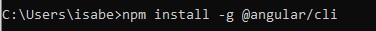
\includegraphics[scale=1]{npmangularcli}
\caption{Instalación de Angular CLI}
\end{figure}
Por último, desde la carpeta que ubica tanto el proyecto del museo (museo-eii) como el de la administración (museo-eii-admin), se ejecuta el comando \textit{npm install} para instalar los paquetes necesarios.
\begin{figure}[H]
\centering
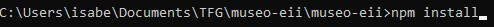
\includegraphics[scale=1]{npminstallmuseo}
\caption{Instalación de los paquetes del proyecto del museo}
\end{figure}
\begin{figure}[H]
\centering
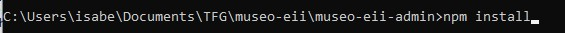
\includegraphics[scale=1]{npminstalladmin}
\caption{Instalación de los paquetes del proyecto de administración}
\end{figure}


\subsection{Manual de Ejecución} 
Una vez completada la instalación siguiendo los pasos descritos en el apartado anterior, se pueden ejecutar ambas aplicaciones utilizando el comando \textit{ng serve -o}, \textit{npm start} o \textit{npm run ng serve -o}. Esto hará que la aplicación esté disponible en \url{http://localhost:4200}.
\begin{figure}[H]
\centering
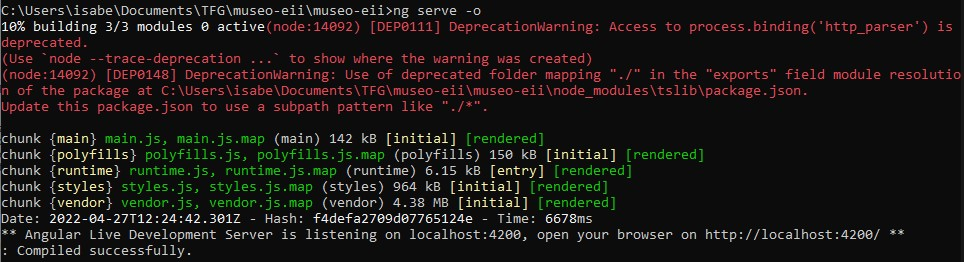
\includegraphics[scale=0.65]{ngservemuseo}
\caption{Ejecución de la aplicación del museo}
\end{figure}
\begin{figure}[H]
\centering
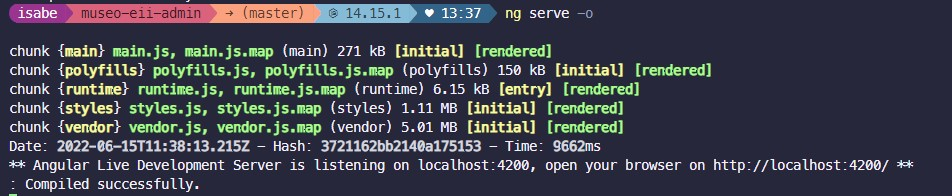
\includegraphics[scale=0.65]{ngserveadmin}
\caption{Ejecución de la aplicación de administración}
\end{figure}


\subsection{Manual de Usuario} 
\subsubsection{Museo}
Al acceder a la web observamos la página de inicio. La parte superior de esta página está presente en toda la aplicación web y, por orden de izquierda a derecha, observamos:
\begin{itemize}
	\item El logo de la escuela, que redirige a esta página de inicio.
	\item Museo, que redirige a la vista general del museo.
	\item Acerca de.
	\item Un selector de idioma, que permite cambiar entre inglés y español.
\end{itemize}
La parte inferior, que contiene enlaces a las redes sociales de la escuela, también está presente en toda la aplicación web.\par
En la parte central se encuentra el contenido específico de la página de inicio: una bienvenida a la página web y un botón que nos dirige a la vista general del museo.
\begin{figure}[H]
\centering
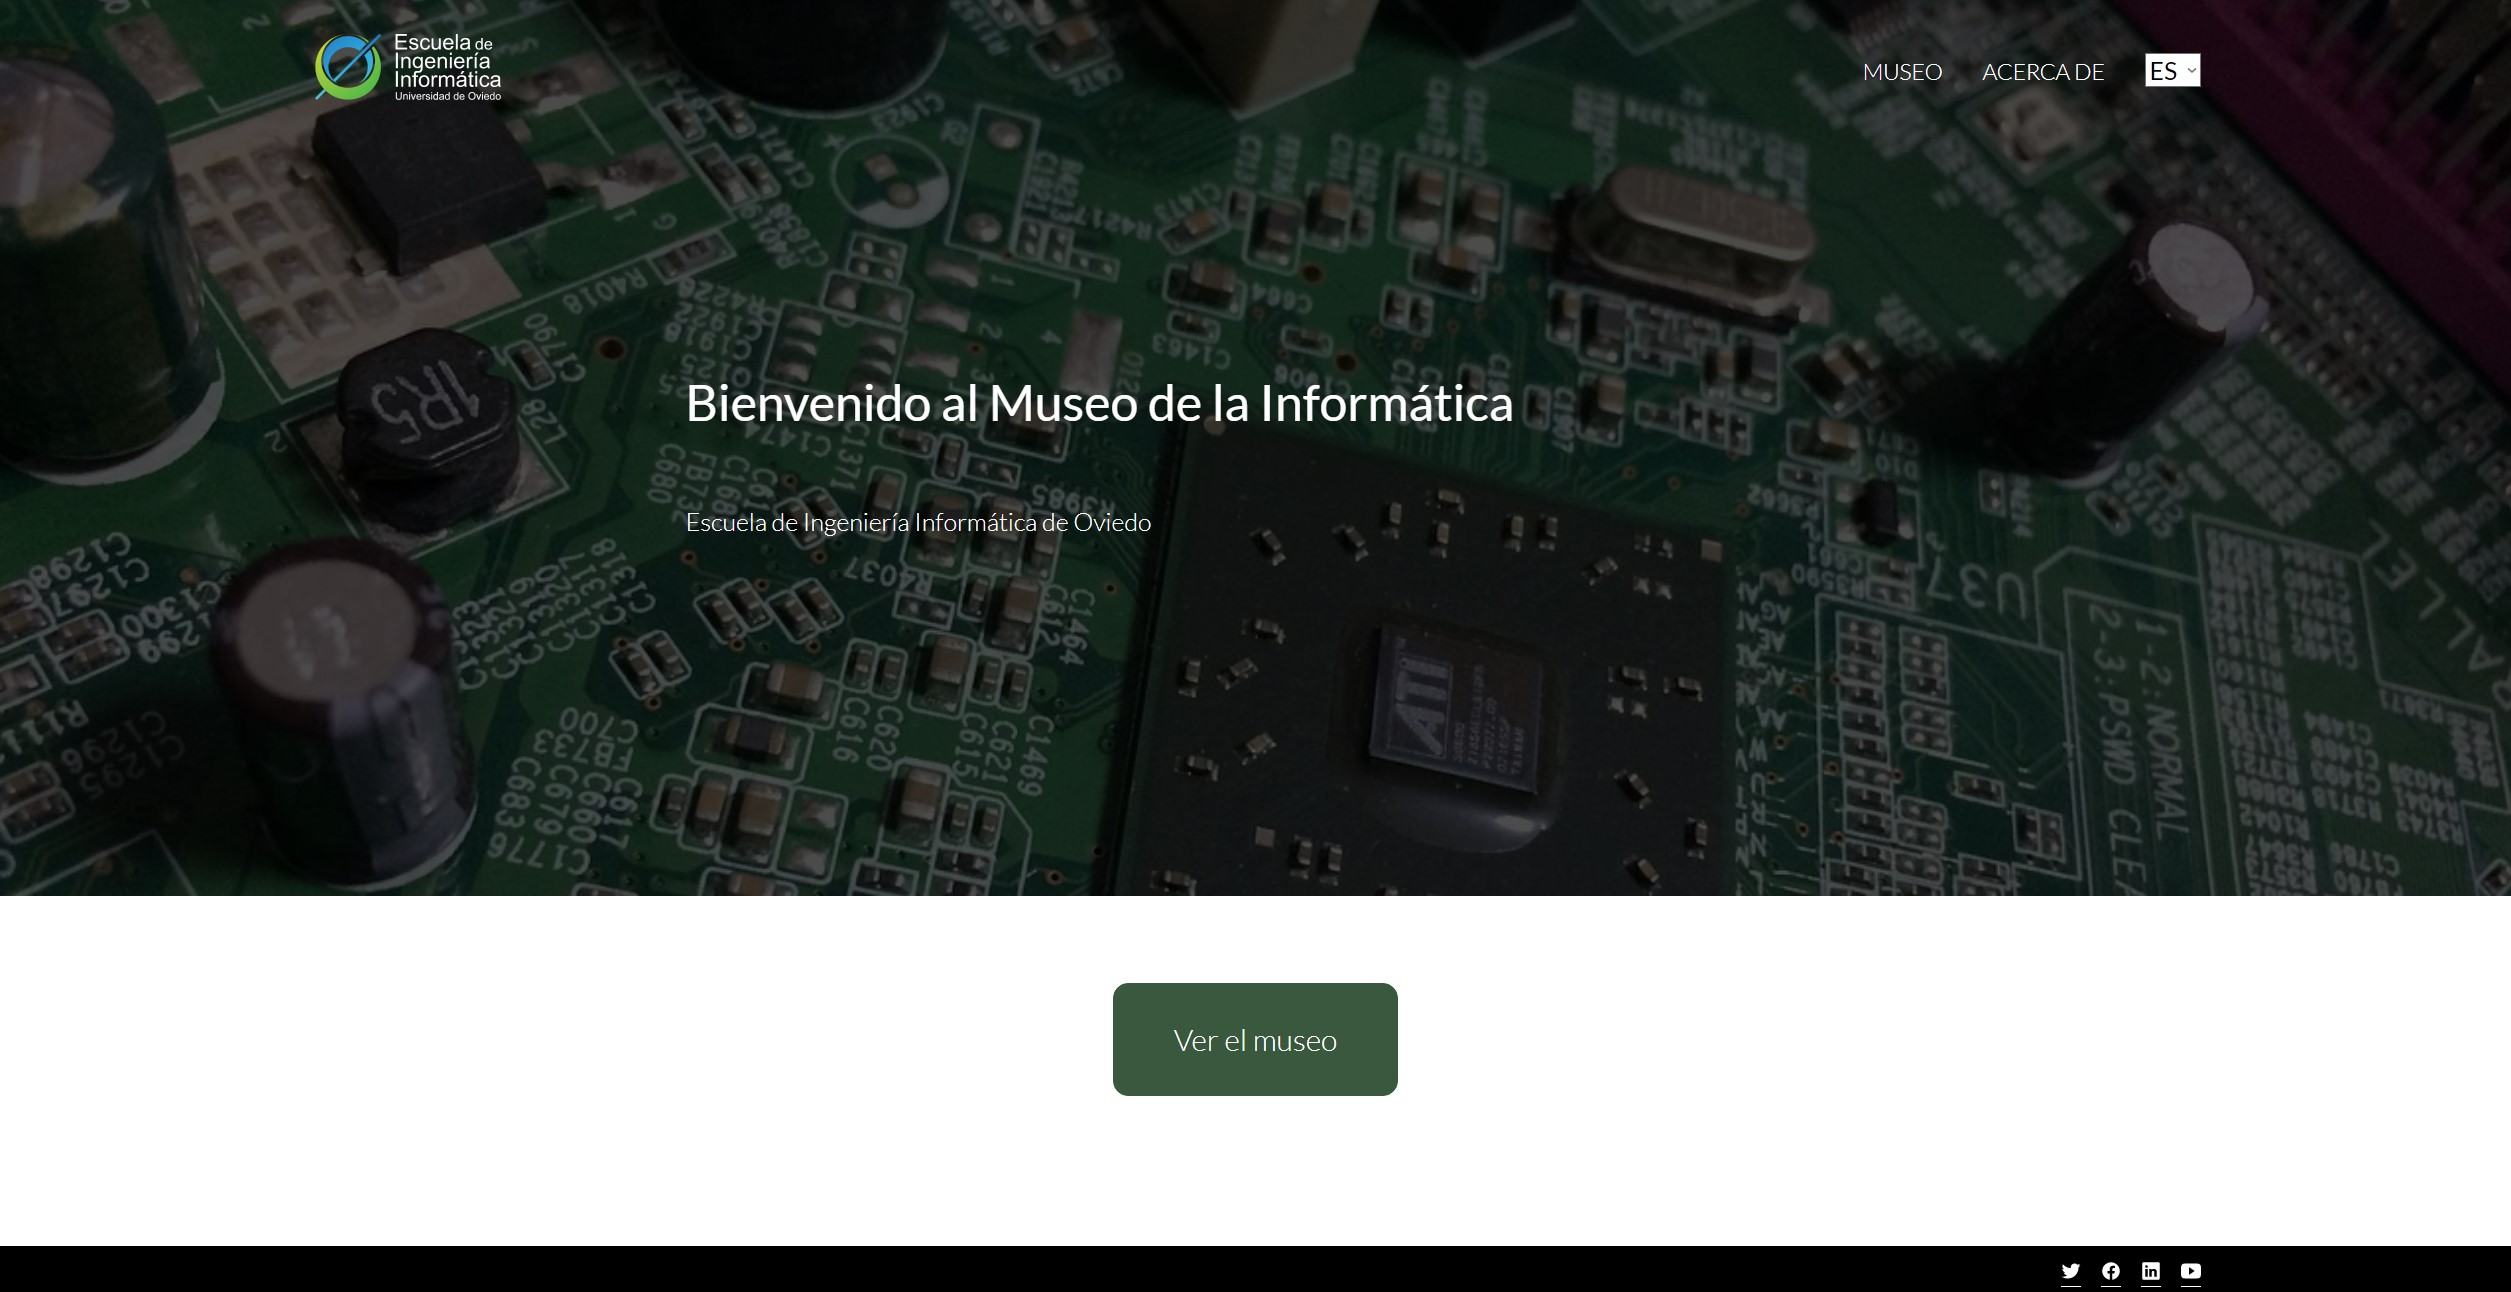
\includegraphics[scale=0.25]{homeIUDef}
\caption{Manual de usuario: Inicio}
\end{figure}
En la vista general del museo hay una línea temporal y filtros de búsqueda.\par
En cada elemento de la línea temporal se muestra el nombre del periodo con un enlace al mismo, los años que comprende dicho periodo, y los nombres de los componentes pertenecientes al periodo, también con enlaces a cada uno de ellos.\par
La búsqueda puede realizarse por años o por nombre. Se puede filtrar por años mediante la barra deslizadora, y se mostrarán entonces todos aquellos periodos que, parcialmente o en su totalidad, tengan componentes pertenecientes a esos años. La búsqueda por nombre se realiza tras escribir en el recuadro de búsqueda y pulsar la tecla \textit{Enter}, y el resultado será aquellos periodos cuyo nombre o el nombre de alguno de sus componentes contenga el texto buscado.
\begin{figure}[H]
\centering
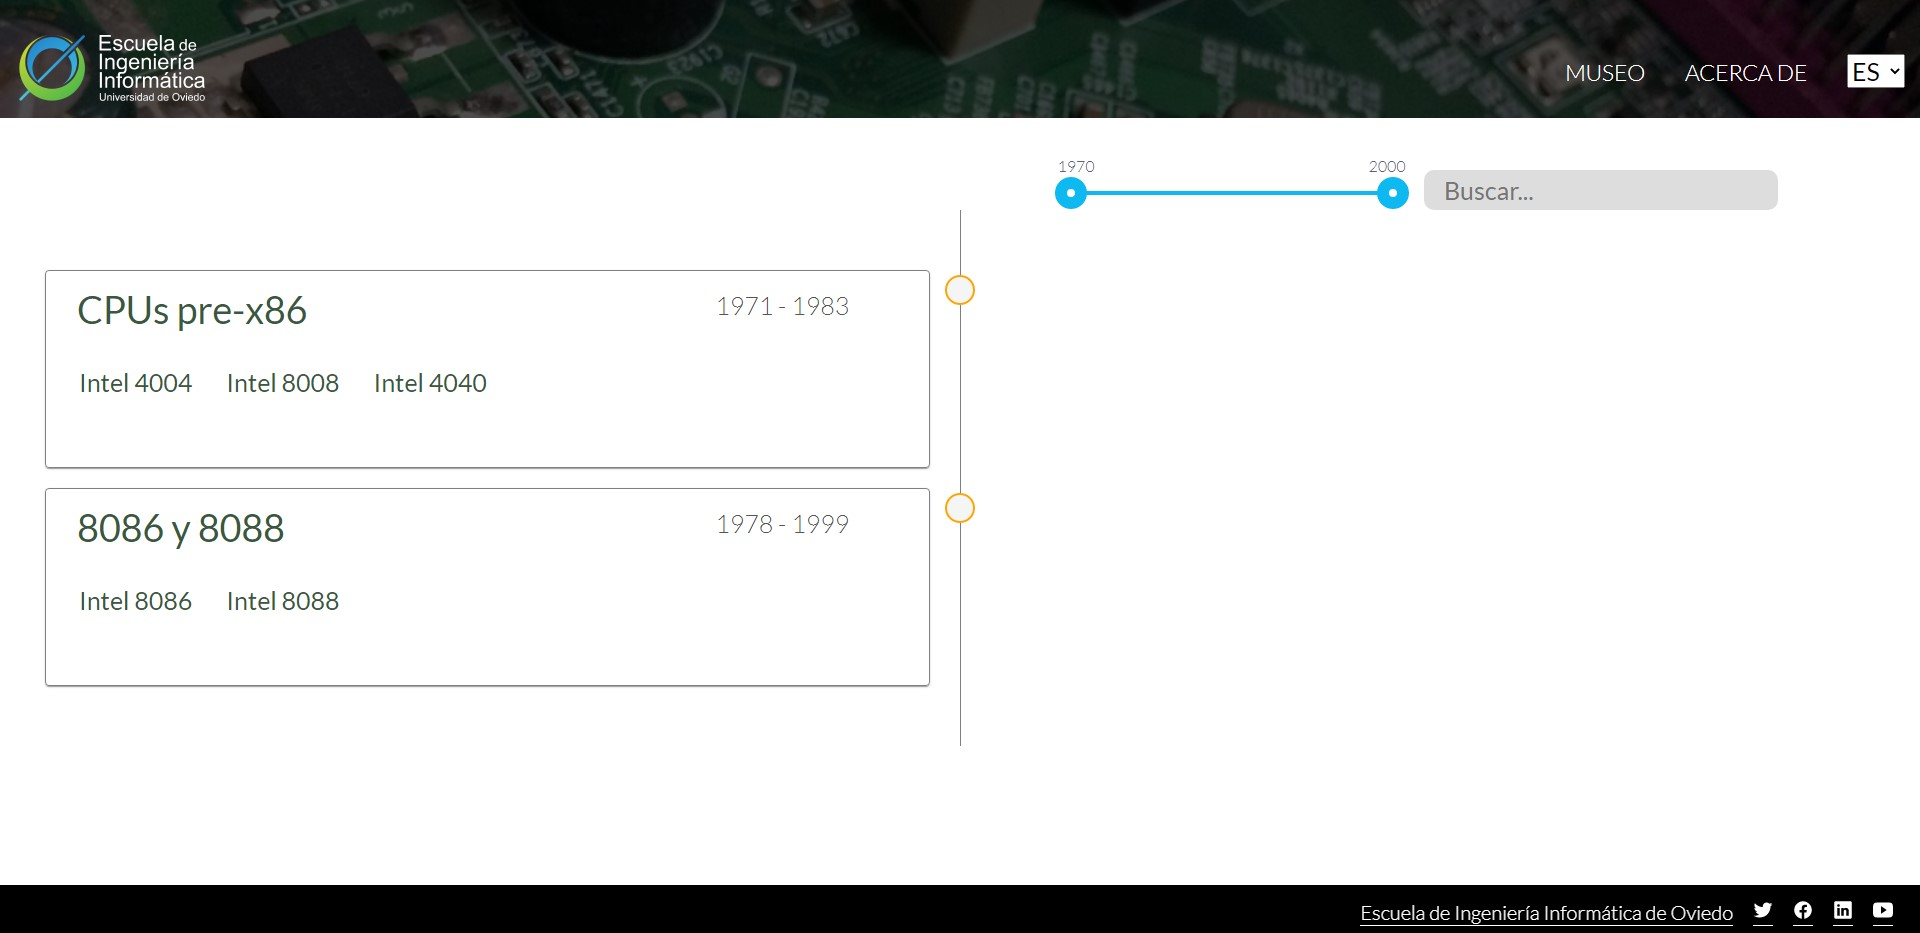
\includegraphics[scale=0.25]{museoIUDef}
\caption{Manual de usuario: Vista general del museo}
\end{figure}
Al entrar en un periodo, en la parte superior podemos ver un menú, en la izquierda se mostraría el periodo anterior cronológicamente, y en la izquierda el periodo siguiente (si existen). El contenido principal de la página son los detalles del periodo: nombre, características, una lista de curiosidades (sabías que...), eventos informáticos ocurridos en esos años, los componentes pertenecientes al periodo (mostrando una imagen y el nombre, con un enlace al componente), y una serie de sistemas famosos que llevan esos componentes. 
\begin{figure}[H]
\centering
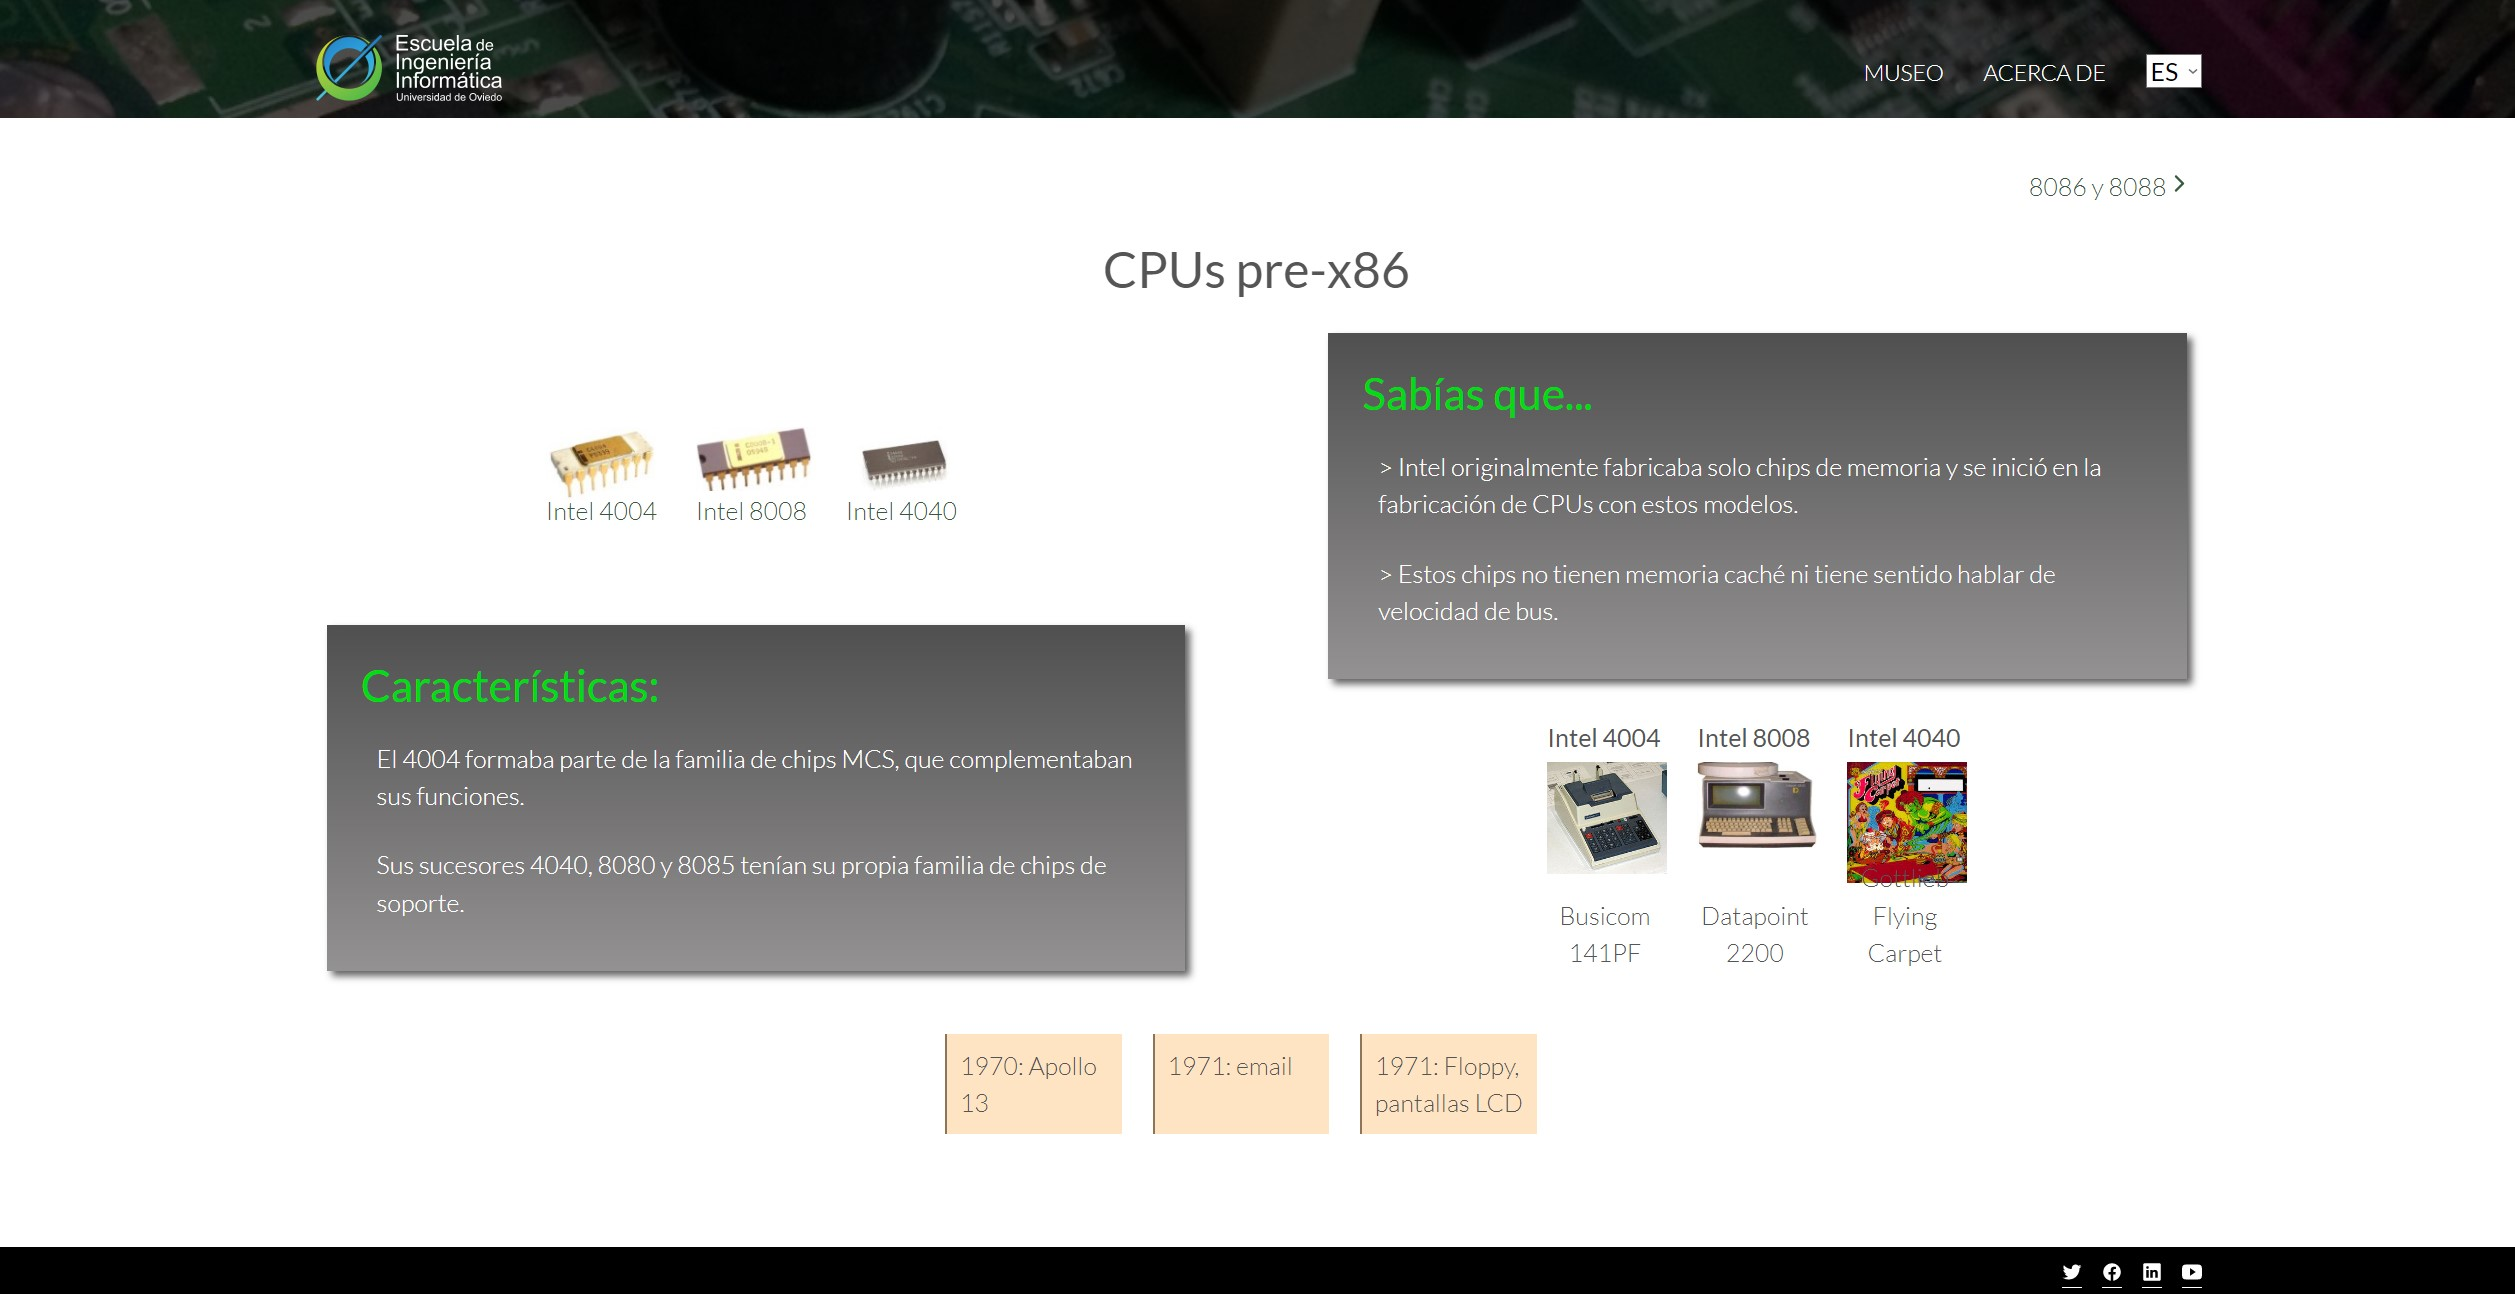
\includegraphics[scale=0.25]{periodoIUDef}
\caption{Manual de usuario: Detalles del periodo (museo)}
\end{figure}
Por último, al acceder a un componente, podemos ver una galería de fotos que se abrirán en grande al pulsar sobre ellas, una descripción del componente y un listado de características. Además, en el lateral izquierdo hay un menú que permite navegar entre periodos (ver el anterior, el actual y el siguiente) y entre los componentes del periodo actual.
\begin{figure}[H]
\centering
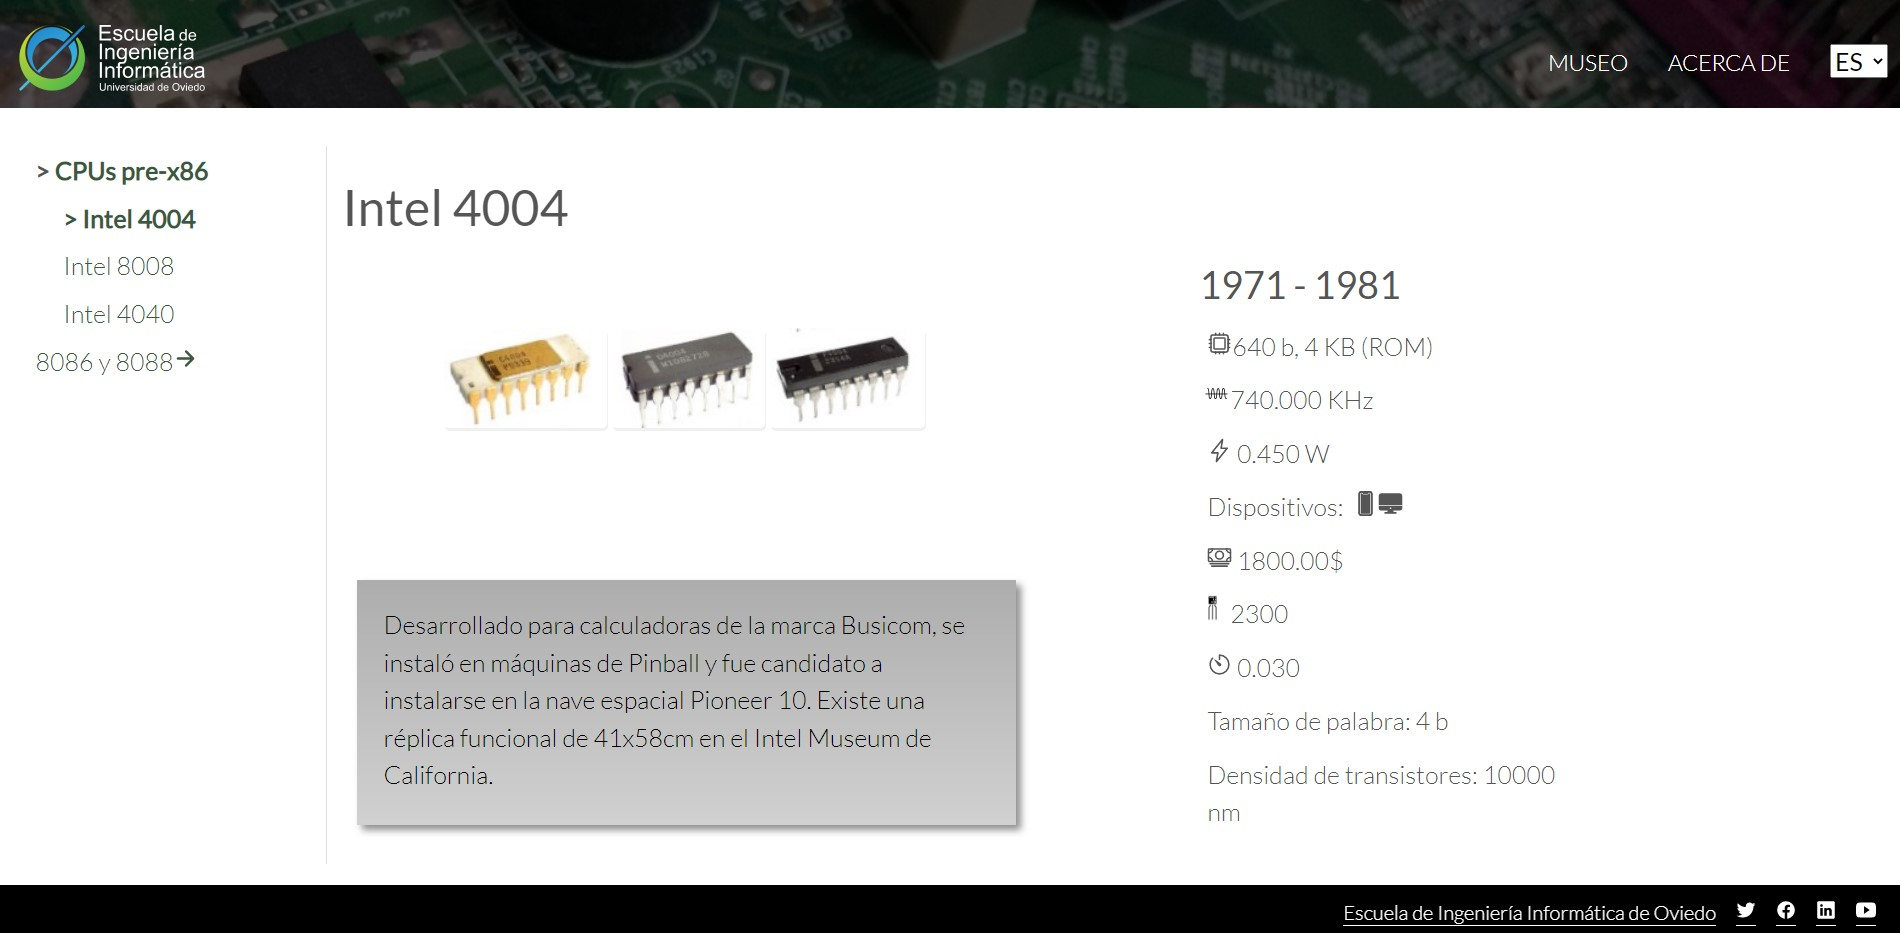
\includegraphics[scale=0.25]{piezaIUDef}
\caption{Manual de usuario: Detalles del componente (museo)}
\end{figure}

\subsubsection{Administración del museo}
Al entrar a la web de administración del museo nos encontramos con el inicio de sesión. Es necesario indicar el correo electrónico y la contraseña para acceder.
\begin{figure}[H]
\centering
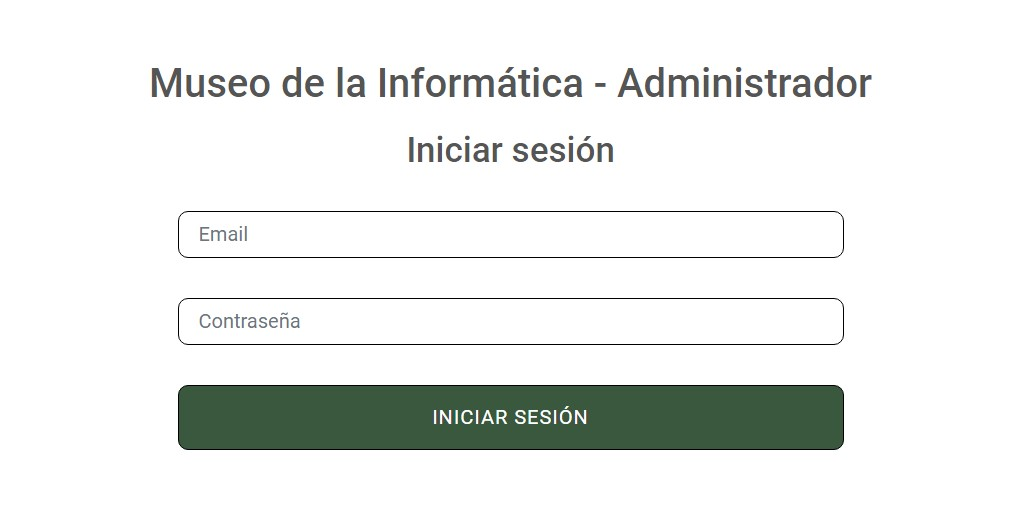
\includegraphics[scale=0.45]{loginIUDef}
\caption{Manual de usuario: Inicio de sesión}
\end{figure}
Lo primero que se muestra una vez iniciada la sesión es un listado de los periodos existentes, mostrando sus nombres con un enlace a cada uno de ellos, y permitiendo editar y eliminar cada periodo. Eliminar un periodo borrará también los componentes asociados al mismo, para ello se mostrará un aviso y se pedirá confirmación. En el lateral izquierdo hay un menú que se incluye en todas las páginas de la aplicación, desde el que se puede acceder a este listado de periodos, y a los formularios para añadir periodos y componentes.
\begin{figure}[H]
\centering

\includegraphics[scale=0.35]{listadoPeriodosIUDef}
\caption{Manual de usuario: Listado de periodos}
\end{figure}
Los detalles de un periodo y del componente muestran los mismos datos explicados anteriormente en el manual de usuario del museo, con la diferencia de en que cada una de estas páginas se muestra una opción para editar el periodo o el componente que estemos visualizando, y en el listado de componentes del periodo también se da la opción de editar o eliminar cada uno de ellos.
\begin{figure}[H]
\centering
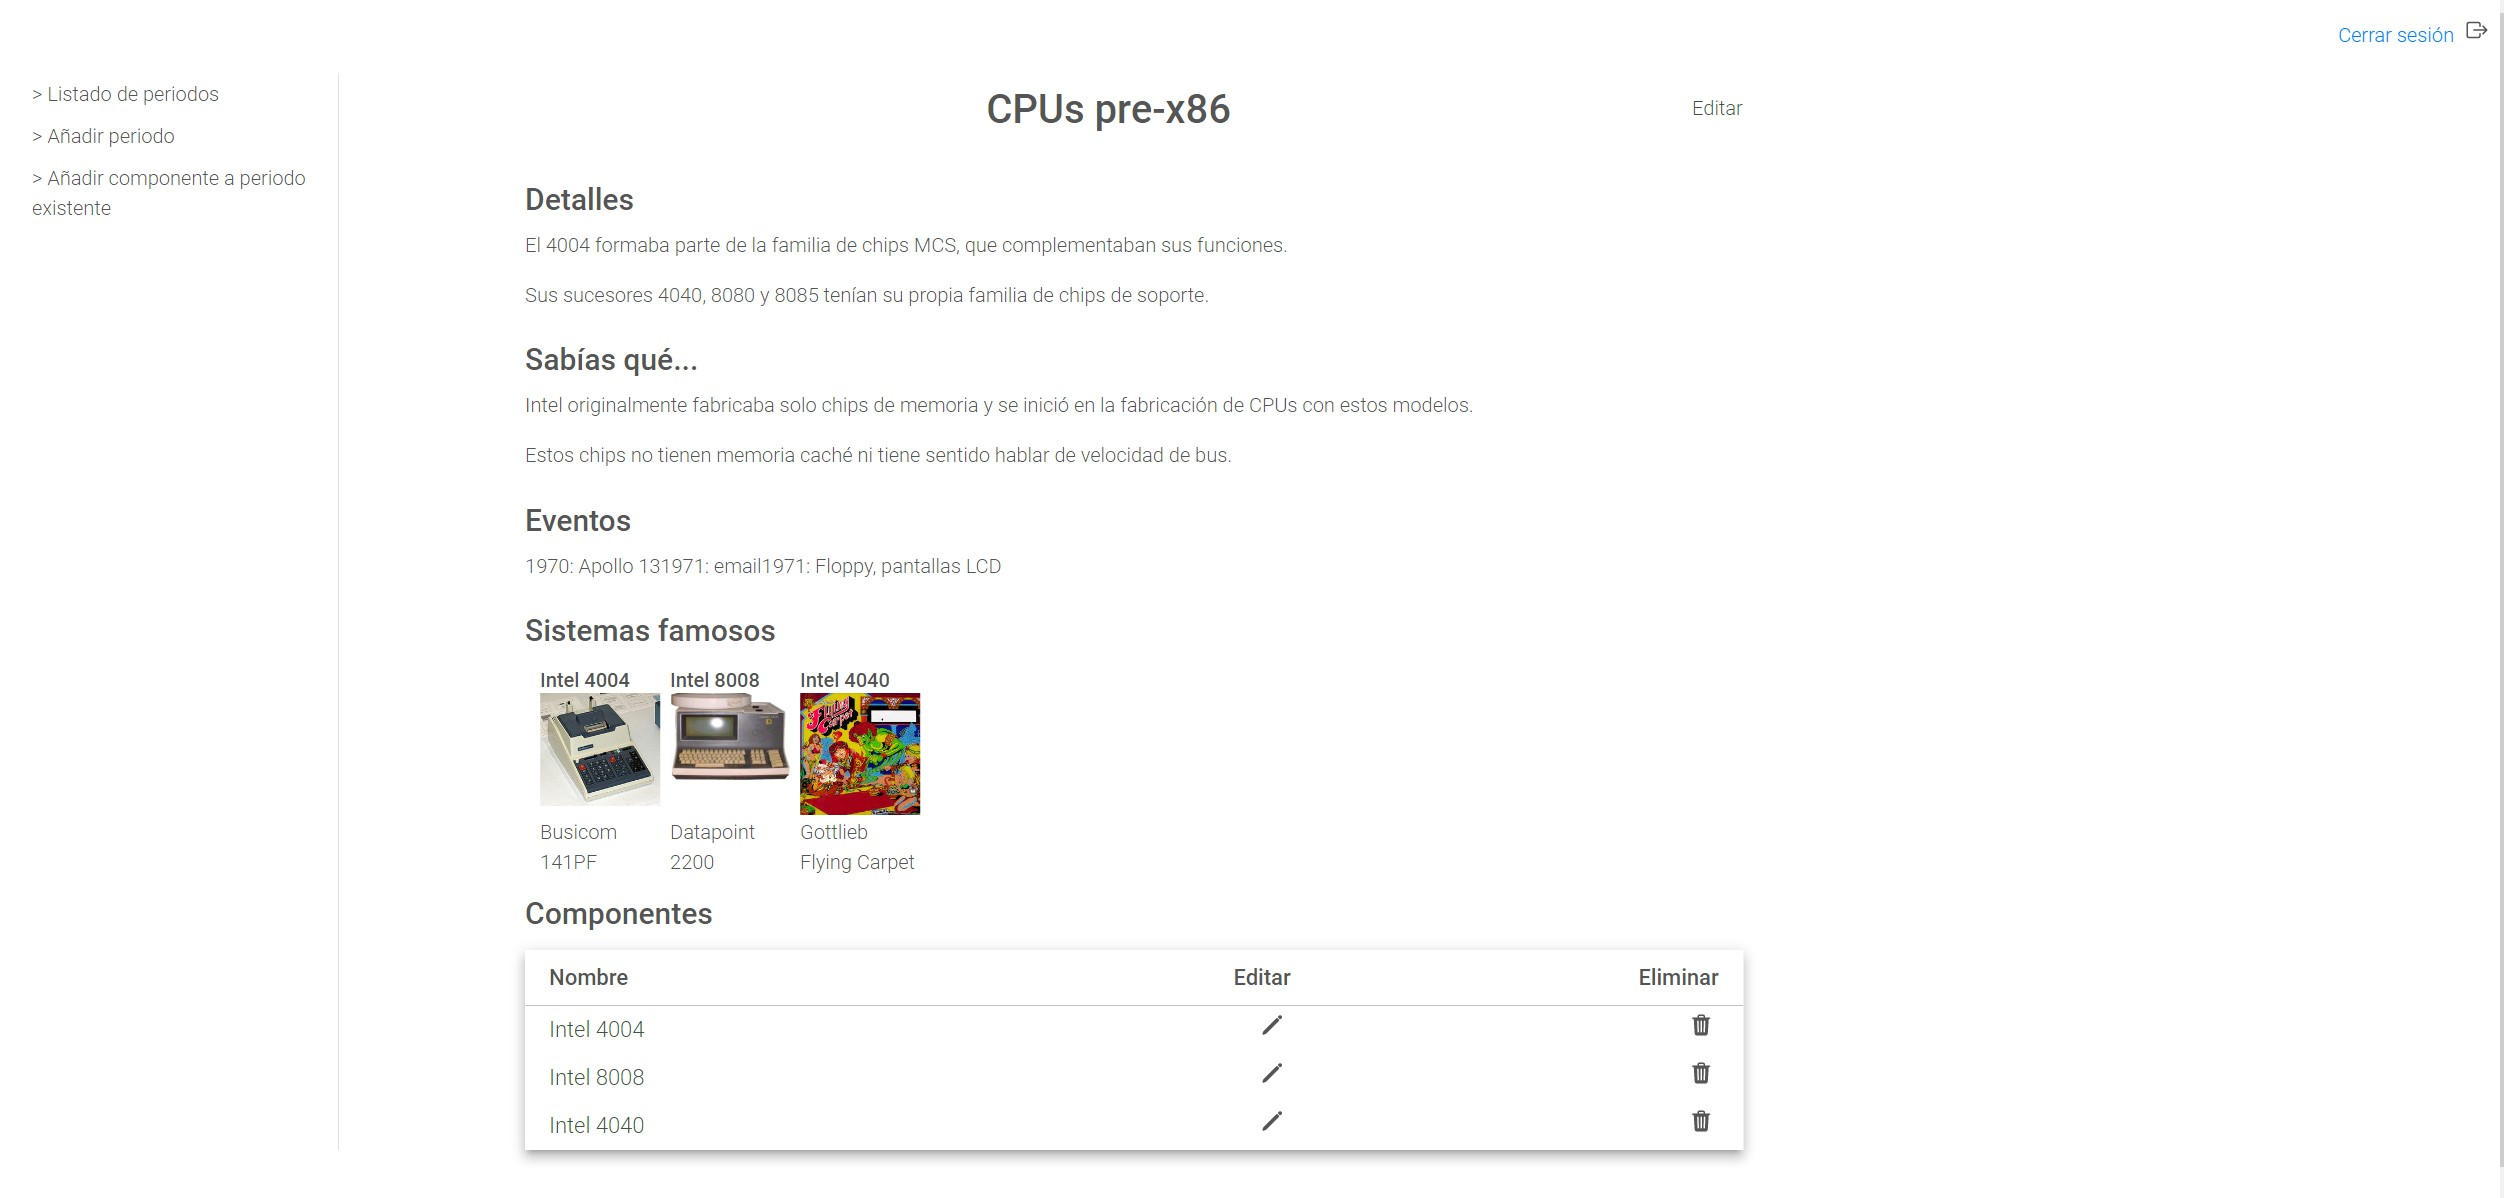
\includegraphics[scale=0.35]{periodoIU2Def}
\caption{Manual de usuario: Detalles de un periodo (administración)}
\end{figure}
\begin{figure}[H]
\centering
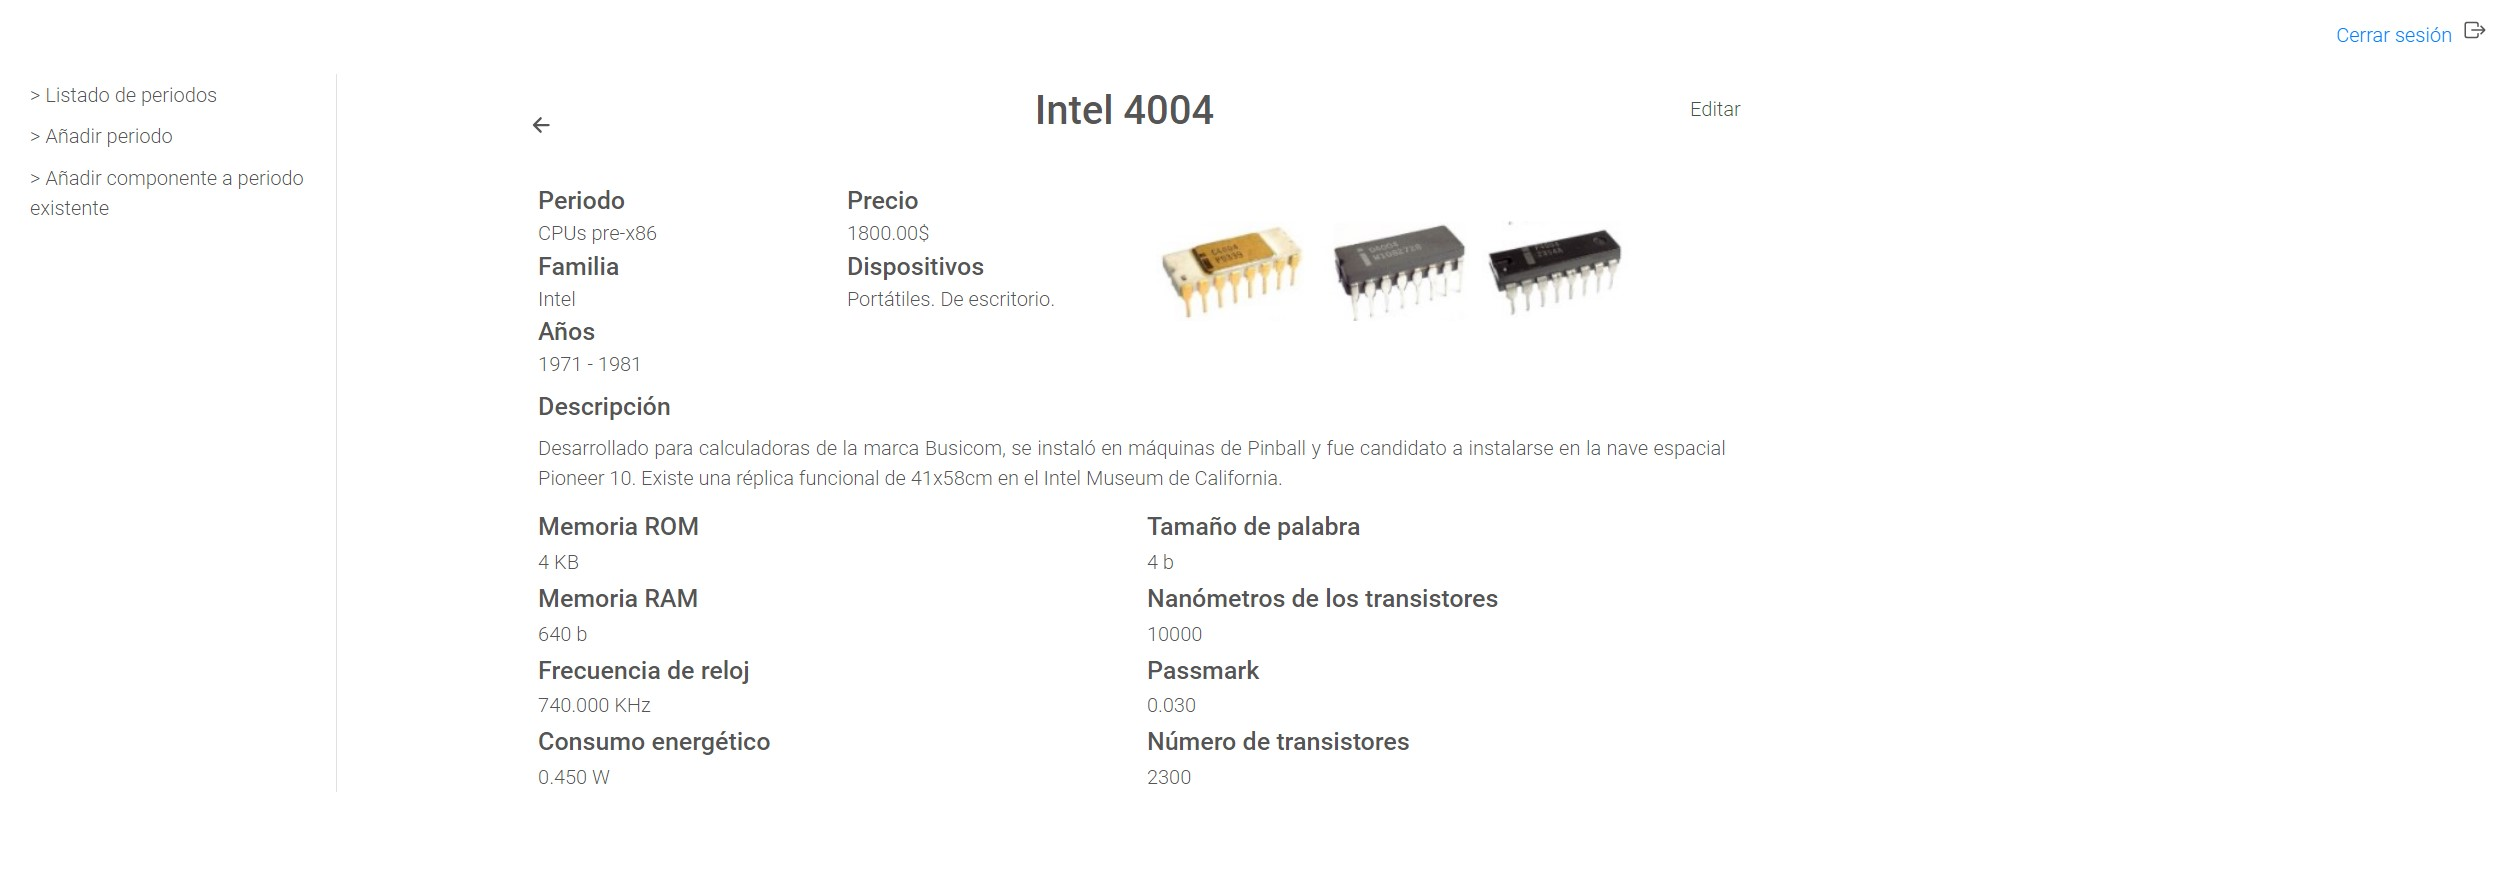
\includegraphics[scale=0.35]{compIUDef}
\caption{Manual de usuario: Detalles de un componente (administración)}
\end{figure}
En el formulario de añadir un periodo hay cuatro entradas de texto para nombre, detalles, curiosidades y eventos del periodo. Todos ellos deben rellenarse obligatoriamente para poder guardar el periodo. Si se pulsa el botón \textit{Cancelar}, el formulario se vaciará de nuevo. Al pulsar \textit{Guardar y continuar} con el formulario completo, se añadirá el periodo a la base de datos del sistema y nos redigirá al formulario para añadir componentes. En cambio, si el formulario no es válido se mostrará un error y no se añadirá.
\begin{figure}[H]
\centering
\includegraphics[scale=0.35]{añadirPeriodoIUDef}
\caption{Manual de usuario: Formulario para añadir un periodo}
\end{figure}
A la hora de editar un periodo, el formulario funcionará igual que al añadirlo, con la diferencia de que los valores iniciales serán los del periodo que se está editando.
\begin{figure}[H]
\centering
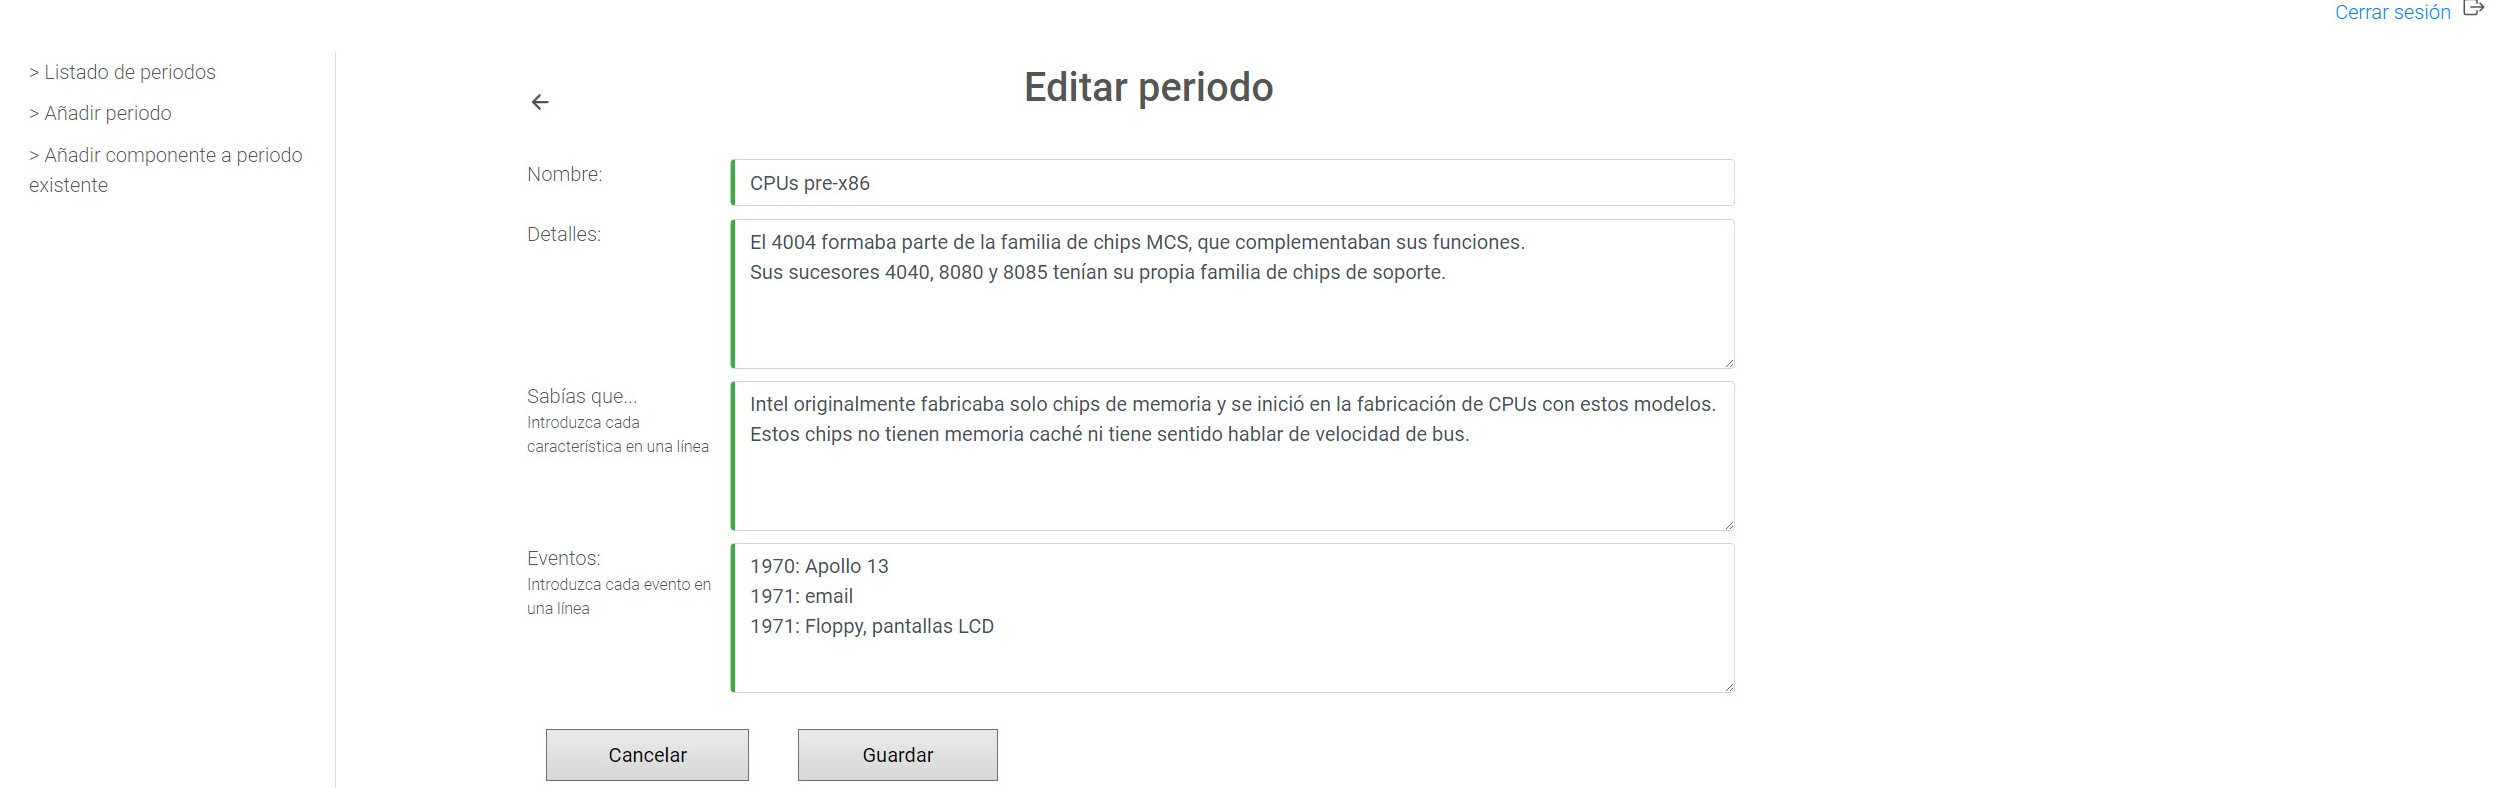
\includegraphics[scale=0.35]{editarPeriodoIUDef}
\caption{Manual de usuario: Formulario para editar un periodo}
\end{figure}
Los formularios para añadir y editar componentes funcionan de la misma forma que los de añadir y editar periodos, pero en este caso, hay campos que no son obligatorios, como la subida de imágenes y el sistema famoso. Además, al añadir o editar componentes se puede seleccionar su tipo: CPU o componente genérico. Al seleccionar CPU se muestran los campos de memoria ROM, memoria RAM, frecuencia de reloj, consumo energético, tamaño de palabra, nanómetros de transistores, passmark y número de transistores.
\begin{figure}[H]
\centering
\includegraphics[scale=0.35]{añadirCompIUDef}
\caption{Manual de usuario: Formulario para añadir un componente}
\end{figure}
\begin{figure}[H]
\centering
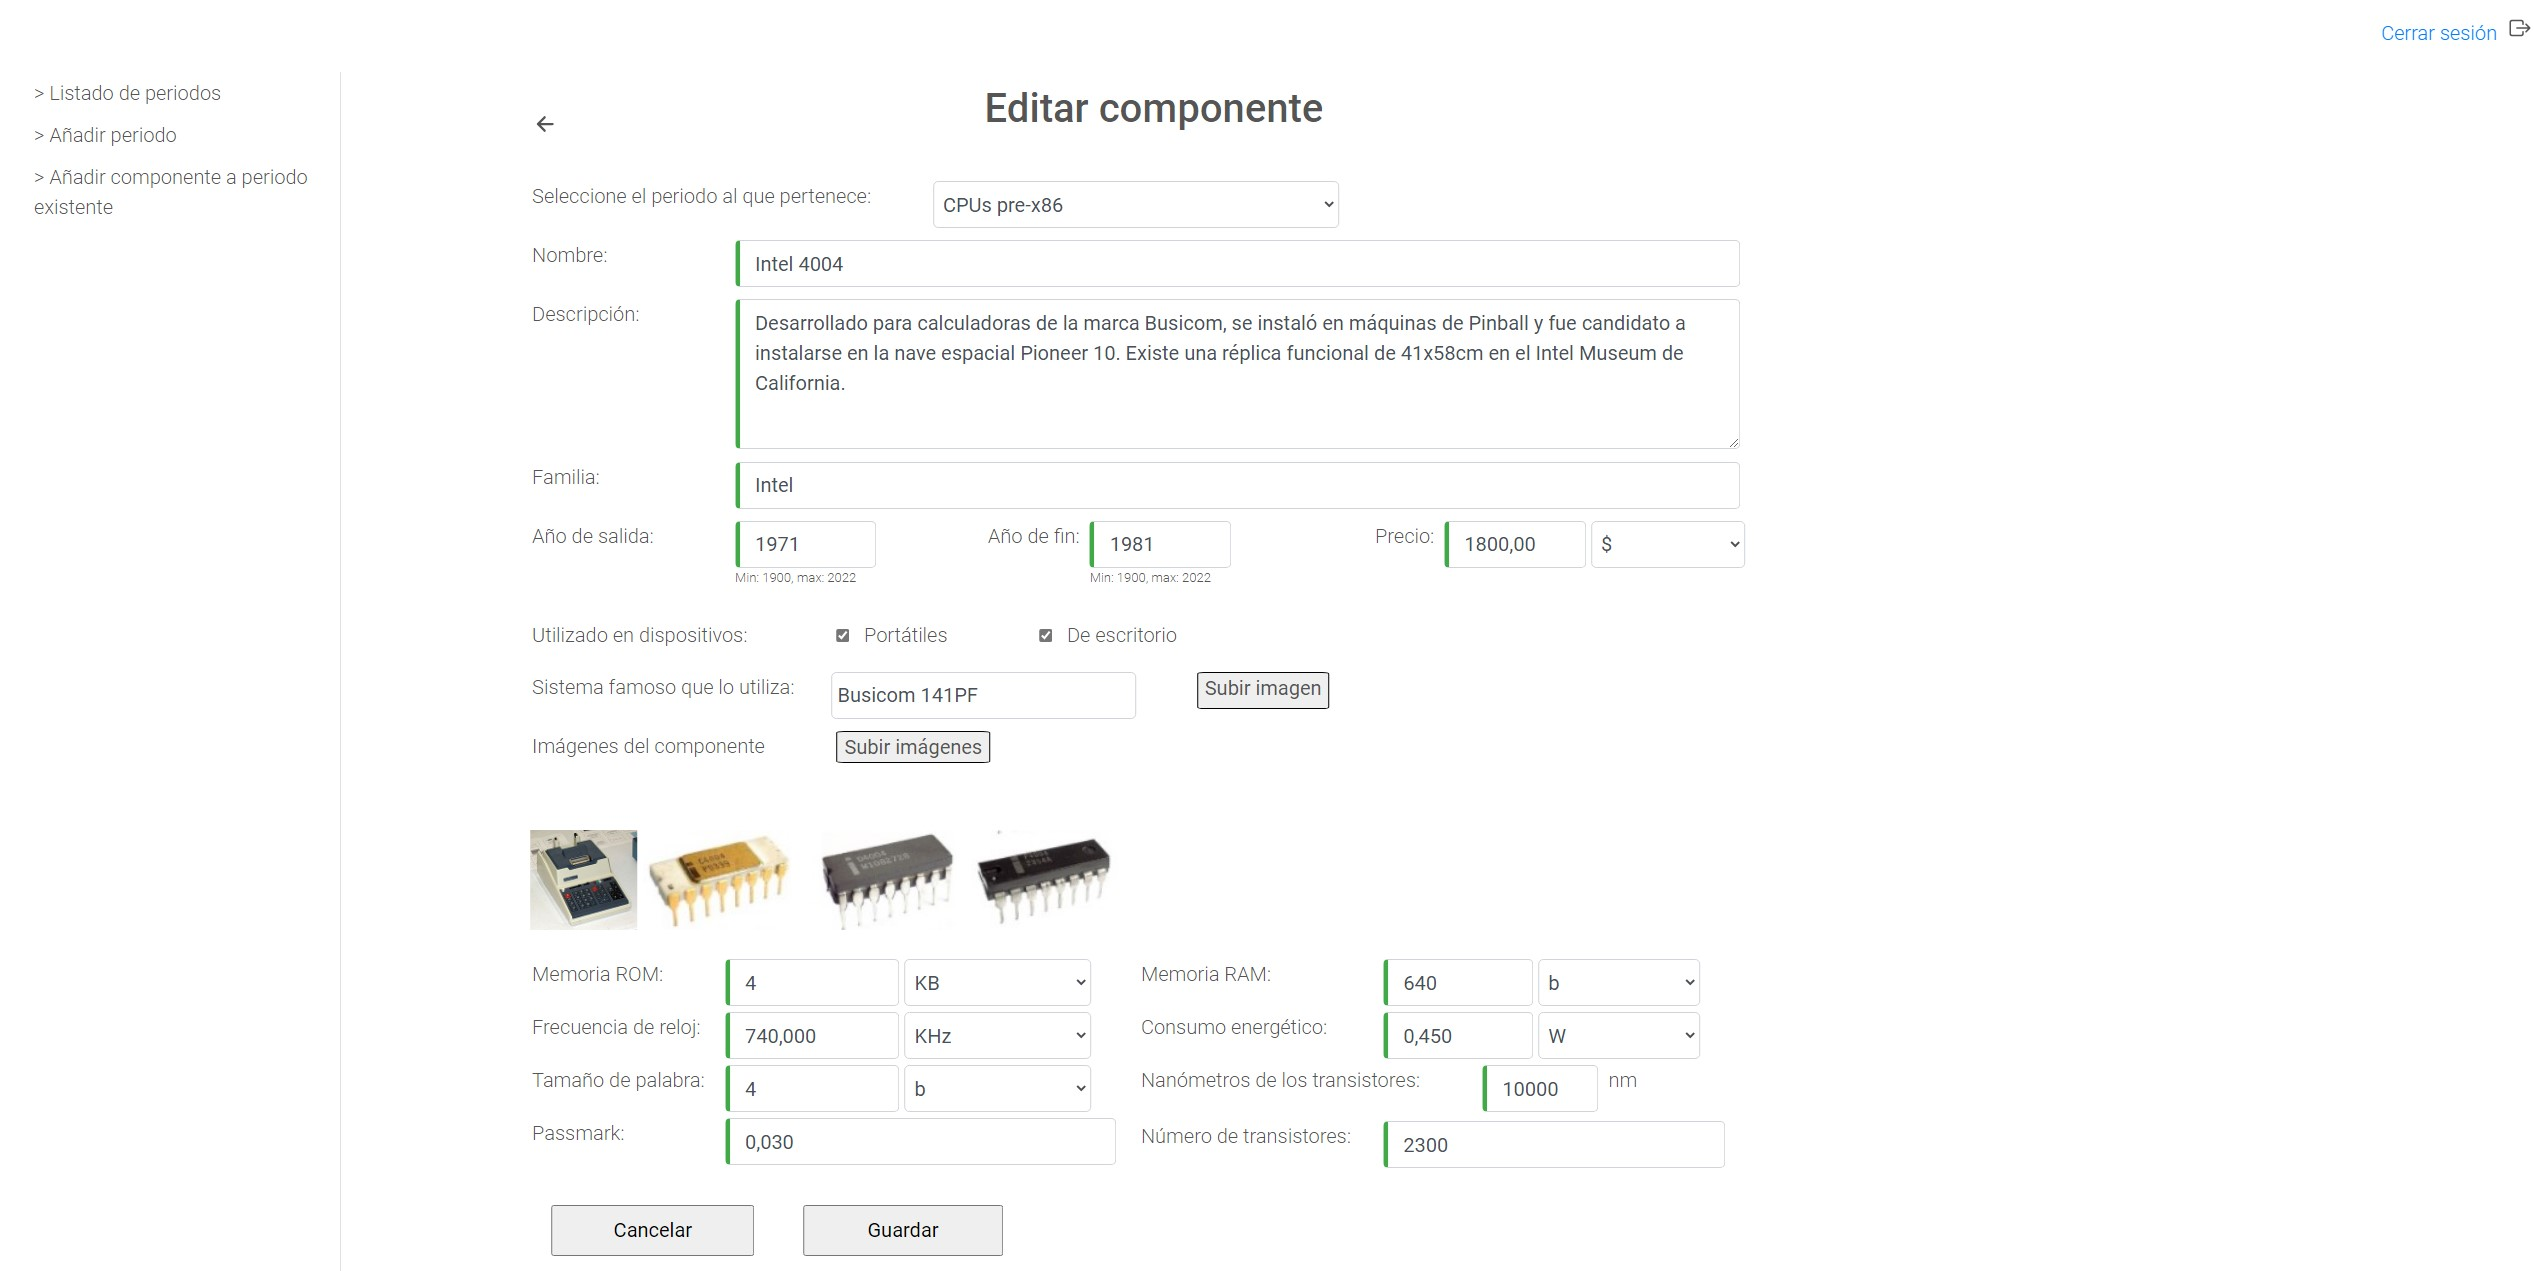
\includegraphics[scale=0.35]{editarCompIUDef}
\caption{Manual de usuario: Formulario para editar un componente}
\end{figure}


\subsection{Manual del Programador}
En este manual se explicará cómo ampliar la aplicación añadiendo nuevos tipos de componentes además de CPUs. Primero habría que crear una nueva clase para cada tipo que se desee añadir. Cada una de estas clases implementarán la interfaz \textit{MyComponent} y heredarán de \textit{GenericComp}. También habría que actualizar la enumeración \textit{CompTypes}. Estos tres elementos mencionados se encuentran en el archivo \textit{comp.ts}, que forma parte tanto del proyecto del museo (museo-eii) como de la administración (museo-eii-admin). Una vez realizado esto, común a ambos proyectos, se explicará qué debe añadirse a cada uno de ellos en específico, así como a la base de datos.

\subsubsection{Museo}
En el proyecto del museo (museo-eii) deberá generarse un componente de Angular para cada tipo añadido, se llamará \textit{`new type`DetailsComponent} y será hijo de \textit{CompDetailsComponent}, del que recibirá como input el atributo \textit{comp}. Este solo se mostrará cuando \textit{comp} sea una instancia del tipo correspondiente a `new type`. En \textit{`new type`-details.component.html} se listarán las características de \textit{comp}.\par
Además, en el método \textit{getComp} de \textit{CompDetailsComponent} habrá que añadir las comprobaciones necesarias para mostrar los nuevos tipos definidos.

\subsubsection{Administración del museo}
En el proyecto de la administración (museo-eii-admin) habrá que generar dos componentes de Angular nuevos por cada tipo añadido: 
\begin{itemize}
\item \textit{`new type`FormComponent}, hijo de \textit{AddCompComponent} y de \textit{EditCompComponent}. De ambos recibe como input el atributo \textit{model}. En \textit{`new type`-form.component.html} se incluirán los campos del formulario que se correspondan con las características del tipo creado. Se mostrará cuando \textit{model} sea una instancia del tipo correspondiente a `new type`. \par
En el método \textit{createModel} de \textit{AddCompComponent} habrá que añadir la opción de crear un objeto de este nuevo tipo, y también se añadirán las comprobaciones necesarias en los métodos \textit{isValid} y \textit{cloneComp} de \textit{AddCompComponent} y \textit{EditCompComponent}.
\item \textit{`new type`DetailsComponent}, hijo de \textit{MyComponentComponent}, del que recibe como input el atributo \textit{c}. En este caso, se hará exactamente lo mismo que lo mencionado anteriormente al añadir \textit{`new type`DetailsComponent} en el proyecto del museo, ya que ambos componentes son para mostrar las características de cada tipo.
\end{itemize}

\subsubsection{Base de datos}
En la base de datos habría que crear una tabla por cada nuevo tipo de componente, con los campos necesarios para este que no estén ya incluidos en la tabla \textit{components}. La clave primaria de esta tabla sería también una clave foránea, el identificador del componente en la tabla \textit{components}. Una vez creadas las tablas correspondientes, habría que modificar las comprobaciones y consultas realizadas en los archivos \textit{getComp.php, updateComp.php} y \textit{postComp.php} para incluir los nuevos tipos creados.


%\newpage
%\section{CSI 8: CONSTRUCCIÓN DE LOS COMPONENTES Y PROCEDIMIENTOS DE MIGRACIÓN Y CARGA INICIAL DE DATOS}


